\chapter{Pilot User Study} \label{sec:userstudy}

\section{Pilot Study Motivation and Goals}
	Aside from creating an interface for simulations and analysis, I also made preparations for a pilot user study aimed at answering a few evaluation questions about the usability of our online interface.
	Specifically the first question we are looking to answer is whether OASIS is accessible.
	The second question we are looking to answer is whether OASIS is an easy to use interface for both novices and users with relevant modeling experience.
	Lastly, we are investigating if OASIS is a step the in the right direction as an early design tool for daylighting analysis.
	In addition to questions pertaining to the online interface's usability, I am also interested in analyzing the perceived accuracy of the physical sketch interpretation algorithm when using non-physical sketches.
	Furthermore, I would also like to collect qualitative feedback on users' understanding of simulation results.
	Also, I would like to analyze the general performance of our system;
	As an early design tool it is imperative that we deliver both sketch interpretations and model renderings quickly.
	Our eventual goal is that OASIS will be an iterative design tool for creativity solving daylighting problems and exploring initial designs with a minimal cost of effort.
	Moreover, the hope is that this pilot user study will provide us valuable feedback to improve OASIS as an early design tool for daylighting.\\

\section{Previous User Studies}
	The physical sketch interpretation algorithm has gone through three previous user studies \cite{cutler2010interpreting,nasman2013evaluation}.
	Two of those studies are direct elevations of the physical sketch interpretation algorithm's accuracy on physical sketches.
	These two studies are featured in \textit{Interpreting Physical Sketches as Architectural Models}\cite{cutler2010interpreting}.
	The first study aims at analyzing the range of designs possible with physical sketches on the Virtual Heliodon.
	The second study aims at analyzing the accuracy of the physical sketch interpretation algorithm on ambiguous sketches.
	In our pilot user study I do not explicitly attempt to analyze the accuracy of the physical sketch interpretation algorithm with non-physical sketches. Yet, I hope that some quantitative feedback will verify that users' intentions are matched at rates similar to these previous studies.
	It is also important to note that while these previous studies gathered over 300 physical sketches, they did so from a medium sized pool of users.
	This pool of users varied from 13 to 30 participants across all previous user studies.
	It is also important to note that these studies each took, on average, 2 months to complete data collection. Moreover, the pool of users these two studies drew upon were comprised of mostly students at Rensselaer Polytechnic Institute.
	Similarly, the \textit{Evaluation Of User Accuracy In A Tangible User Interface For Architecture Design} was comprised of 6 architecture students and 7 non-architecture students. While, I do not expect to match the number of models produced per users, I hope that the overall number of models produced will be both quantitatively larger and from a broader range of users.
	In addition, the accessibility and autonomy of our online interface will make the marginal cost of collecting data per users smaller than the tangible user interface on the Virtual Heliodon.

\section{Accessibility Design for OASIS}
	There were various frameworks considered for OASIS.
	Our requirement of accessibility to a broad range of users, however, limited our choices.
	Software that uses OpenGL, or another graphics libraries, would require installation.
	Having an installer and system requirements would be barrier of entry to participating in our study.
	In addition, trying to support multiple platforms would be time intensive and would increase the marginal cost of adding features to OASIS.
	WebGL and ThreeJS are relatively new graphics libraries that are supported on most modern web browsers.
	The availability of WebGL and our requirement of accessibility led me to make OASIS a web-based application.
	Additional benefits of using a web-based application include having a platform independent framework, no installation process, and globally applied updates.
	Having a web-based application lends itself to using a client-server architecture.
	In OASIS I leverage the server to both service our web page and run computationally expensive processes on behalf of clients.
	Namely, these computational expensive processes are the physical sketch interpretation algorithm and the daylight rendering engine.
	Both of these processes are computed on a specialized lab machine rather then locally on users' machines.
	Our lab machine, unlike most clients running our application, is equipped with an NVidia GeForce GTX 780 graphics card, 64 GB of RAM, and a 12 core processor.
	This makes the CPU-intensive process of the physical sketch interpretation algorithm and GPU-intensive processes of the daylight rendering engine faster then on most client machines.
	Interface related computation rely on the client's machine including the manipulation of 2D images, the creation of rendering request for the server, and the visualizing of 3D models.
	My hope is that leveraging the server to run computational expensive components in OASIS will prevent potential participants from opting out of our pilot user study due to hardware limitations and will provide a homogeneous user experience across all platforms.


\section{User Feedback  Collection in OASIS}

	\begin{figure}
	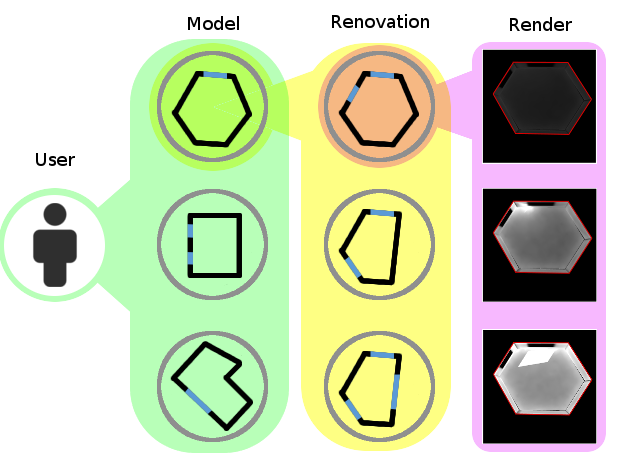
\includegraphics[width=0.8\textwidth]{relationship}
	\caption{Relationship between users, models, renovations, and renderings. Users are associated with a set of models, models are associated with a set of renovations, and renovations are associated with a set of renderings.}
	\label{fig:rel}
	\end{figure}

	In OASIS I collect two types of data from users.
	Both active and passive data are collected from users while they use our tool.
	Active data refers to the feedback, models, and comments user actively provide.
	Passive data refers to data not actively provided by users, such as the length of time a user spends on a page, the average wait time before rendering request are handled, and other information about users usage of our application. We collect both types of data to get a clearer idea of how users perceive OASIS and how users interact with our tool.

	The active feedback data collected from users can be organized as either user-specific questions, model-specific questions, renovation-specific questions, and render-specific questions.
	User-specific questions refer to questions associated with users.
	For example questions pertaining to user's past experience and education.
	User-specific questions also include questions that ask users about their subjective opinion of certain components of OASIS.
	All user-specific questions as well as all feedback questions can be viewed in the appendix. 
	Model-specific questions refer to questions about user created models.
	Model-specific questions include asking users to elaborate on specific models and asking users to rate how confident they are regards to their accuracy of creating models.
	OASIS allows users to make multiple renovations on previously created models.
	Some of the questions I ask are renovation-specific, such as if the physical sketch interpretation algorithm correctly matches users' intentions on a specific renovation of a model.
	Lastly, users can run several renderings per renovation.
	As a result I also ask users renovation-specific questions.
	The relationship between users, models, renovations, and renderings can be seen in Figure-\ref{fig:rel}.
	As mentioned before we also collect passive data.
	Specifically, we collect how long users spend on each page of our interface and how long users wait for both physical sketch interpretations and daylight renderings.



\section{Data Collection}
	In order to collect feedback on OASIS we have to first host the application online, and then bring potential users' attention to the application.
	As with an study, we must invite users to participate in order to collect feedback.
	Personally inviting individuals to use our tool might be cumbersome and slow going, so we hope inviting users in mass via popular social media networks, such as Facebook and Reddit, will result in increased user participation.
	One advantage of using social media networks is that some organized by users' interest. 
	We use this organization to target users who might have an interest in daylighting or architecture.
	Figure-\ref{fig:reddit} list a few relevant Reddit communities and their respective sizes that we plan to advertise OASIS to.

	\begin{table}[h!]
	\centering
	    \begin{tabular}{ | l | l | }
	        \hline
		    Reddit Forum             & Subscribers  \\ \hline
		    Beta 					& 10,1455       \\ \hline
		    InteriorDesign 			& 78,750        \\ \hline
		    RPI 			        & 3,939         \\ \hline
		    Floorplan    			& 1,175         \\ \hline
		    UserExperienceDesign    & 1,128         \\ \hline
		    GreenArchitecture 		& 607          \\ \hline
		    YoungArchitects 		& 236          \\ \hline
	    \end{tabular}
	\end{table}

	Additionally, many feedback questions asked pertain to users creating models of Rensselaer Polytechnic Institute.
	We plan our advertising our tool on campus as well as online.
	As done in previous studies we wish to leverage the Rensselaer Polytechnic Institute School of Architecture in order to collect feedback from users with formal education in Architecture.
	Again, we plan to use user feedback collected both actively and passively to analyze if OASIS is accessible to a wide range of users.
	In addition, we plan to use the feedback to investigate the usability of our online interface.
	Lastly, we want to use collected qualitative user feedback to review if OASIS is a step in the right direction as an early design tool.


